\documentclass[tikz,border=12pt]{standalone}
\usepackage{tikz}
\usetikzlibrary{shapes.geometric, arrows.meta, positioning, calc}
\usepackage{xcolor}

% Define colors
\definecolor{loadcolor}{RGB}{66, 133, 244}
\definecolor{processcolor}{RGB}{52, 168, 83}
\definecolor{decisioncolor}{RGB}{251, 188, 4}
\definecolor{verifycolor}{RGB}{234, 67, 53}
\definecolor{outputcolor}{RGB}{138, 43, 226}

\begin{document}
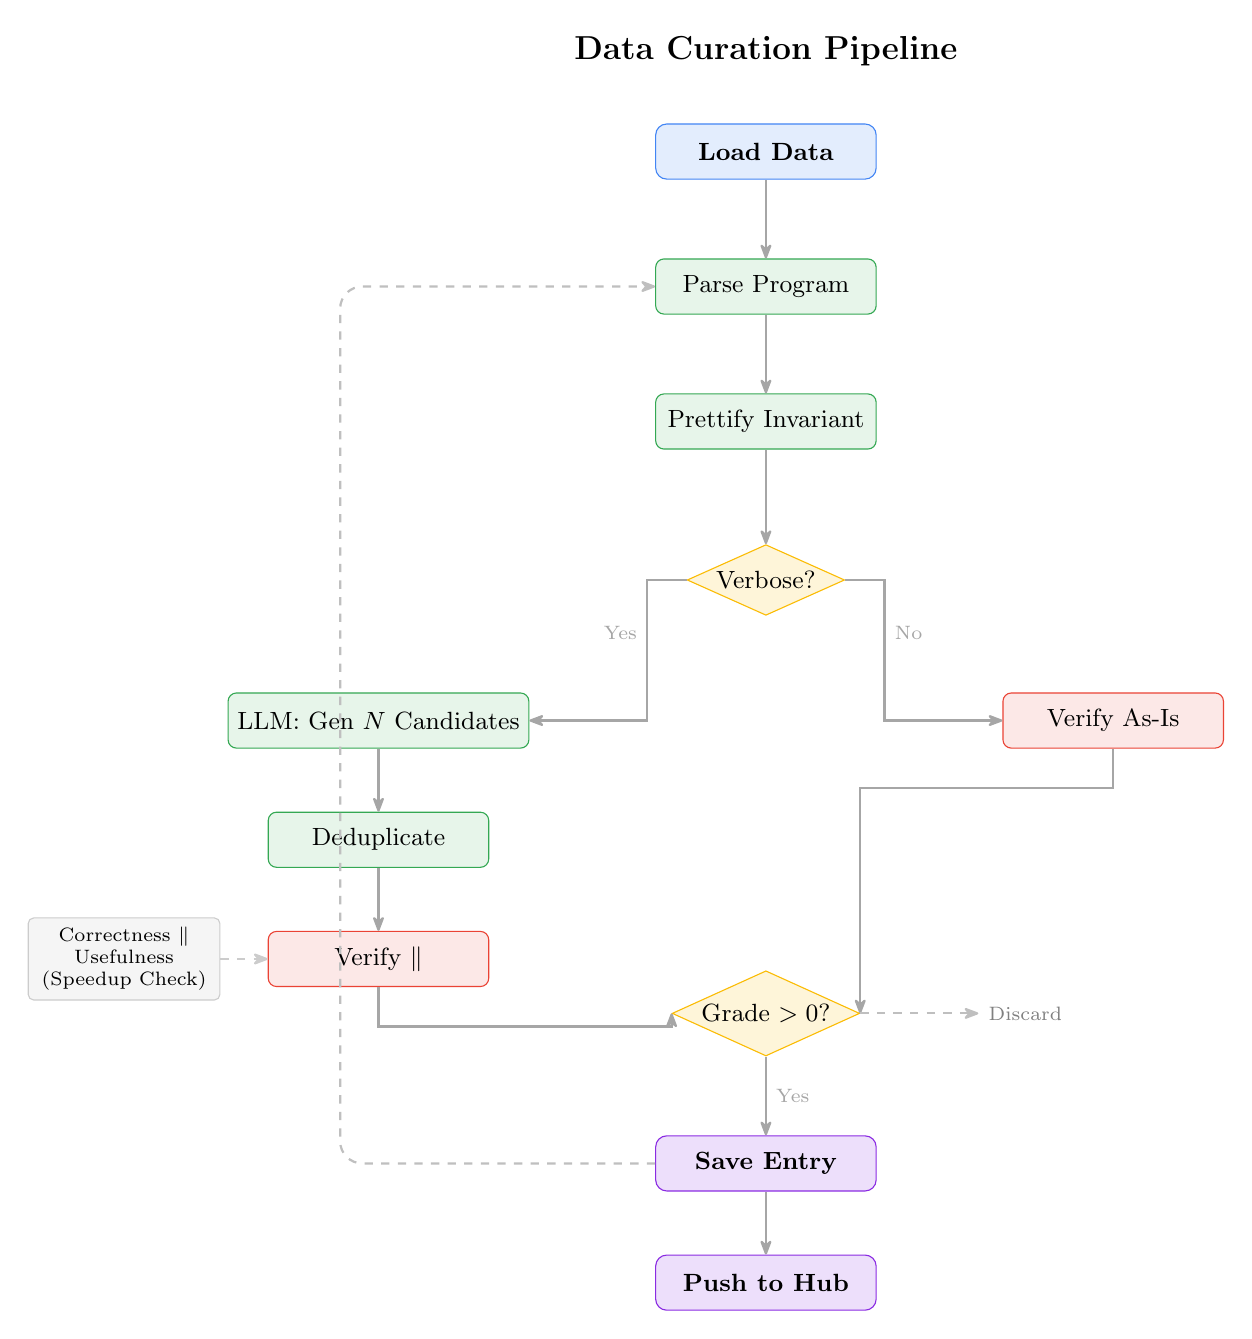
\begin{tikzpicture}[
    node distance=1cm and 2cm,
    >={Stealth[round]},
    % Node styles
    startstop/.style={rectangle, rounded corners=4pt, minimum width=2.8cm, minimum height=0.7cm, text centered, draw=loadcolor, fill=loadcolor!15, font=\small\bfseries},
    process/.style={rectangle, rounded corners=3pt, minimum width=2.8cm, minimum height=0.7cm, text centered, draw=processcolor, fill=processcolor!12, font=\small},
    decision/.style={diamond, aspect=2.2, minimum width=2cm, inner sep=1pt, text centered, draw=decisioncolor, fill=decisioncolor!15, font=\small},
    verify/.style={rectangle, rounded corners=3pt, minimum width=2.8cm, minimum height=0.7cm, text centered, draw=verifycolor, fill=verifycolor!12, font=\small},
    output/.style={rectangle, rounded corners=4pt, minimum width=2.8cm, minimum height=0.7cm, text centered, draw=outputcolor, fill=outputcolor!15, font=\small\bfseries},
    note/.style={rectangle, rounded corners=2pt, draw=gray!40, fill=gray!8, font=\scriptsize, text width=2.2cm, align=center},
    % Arrow styles
    arrow/.style={->, thick, color=gray!70},
    dasharrow/.style={->, thick, dashed, color=gray!50},
]

% Main vertical flow
\node (load) [startstop] {Load Data};
\node (parse) [process, below=of load] {Parse Program};
\node (prettify) [process, below=of parse] {Prettify Invariant};
\node (verbose) [decision, below=1.2cm of prettify] {Verbose?};

% Left branch - Verbose path
\node (llm) [process, below left=1.2cm and 2.5cm of verbose] {LLM: Gen $N$ Candidates};
\node (dedup) [process, below=0.8cm of llm] {Deduplicate};
\node (verpar) [verify, below=0.8cm of dedup] {Verify $\parallel$};

% Right branch - Non-verbose path
\node (verasis) [verify, below right=1.2cm and 2.5cm of verbose] {Verify As-Is};

% Filter (centered below verbose)
\node (filter) [decision, below=4.5cm of verbose] {Grade $> 0$?};

% Output nodes
\node (save) [output, below=1cm of filter] {Save Entry};
\node (hub) [output, below=0.8cm of save] {Push to Hub};

% Arrows - Main flow
\draw [arrow] (load) -- (parse);
\draw [arrow] (parse) -- (prettify);
\draw [arrow] (prettify) -- (verbose);

% Branch arrows with labels
\draw [arrow] (verbose.west) -- ++(-0.5,0) |- node[above left, pos=0.25, font=\scriptsize] {Yes} (llm.east);
\draw [arrow] (verbose.east) -- ++(0.5,0) |- node[above right, pos=0.25, font=\scriptsize] {No} (verasis.west);

% Verbose path flow
\draw [arrow] (llm) -- (dedup);
\draw [arrow] (dedup) -- (verpar);

% Connect both paths to filter
\draw [arrow] (verpar.south) -- ++(0,-0.5) -| (filter.west);
\draw [arrow] (verasis.south) -- ++(0,-0.5) -| (filter.east);

% Output flow
\draw [arrow] (filter) -- node[right, font=\scriptsize] {Yes} (save);
\draw [arrow] (save) -- (hub);

% Discard arrow
\draw [dasharrow] (filter.east) -- ++(1.5,0) node[right, font=\scriptsize, text=gray] {Discard};

% Loop back arrow
\draw [dasharrow, rounded corners=8pt] (save.west) -- ++(-4,0) |- (parse.west);

% Verification detail note (positioned to the left of verpar)
\node[note, left=0.6cm of verpar] (verdetail) {Correctness $\parallel$\\Usefulness\\(Speedup Check)};
\draw [dasharrow, gray!40] (verdetail.east) -- (verpar.west);

% Title
\node[above=0.6cm of load, font=\large\bfseries] {Data Curation Pipeline};

\end{tikzpicture}
\end{document}
